% !TeX spellcheck = en_US
\newpage
\section{Network}
The idea behind the network layer is to \textbf{interconnect} all the LANs, MANs and WANs. To do that it's necessary to introduce uniform internetwork addresses in an end-to-end packet format, abstracting the lower layers and creating a common format that's \textbf{independent} of intermediate link layer technologies.\\
This brings also the necessity to do:
\begin{itemize}
	\item \textbf{Routing}: automatically acquiring and updating next hop information for each destination
	\item \textbf{Forwarding}: moving incoming packets from the input interface to the appropriate output
\end{itemize}

\noindent The main \textbf{goal} of the network layer is to manage end-to-end connectivity across multiple networks. To do that it defines:
\begin{itemize}
	\item Internetwork identifiers
	\item Uniform end-to-end packet
	\item Routing and forwarding mechanisms
\end{itemize}
\begin{center}
	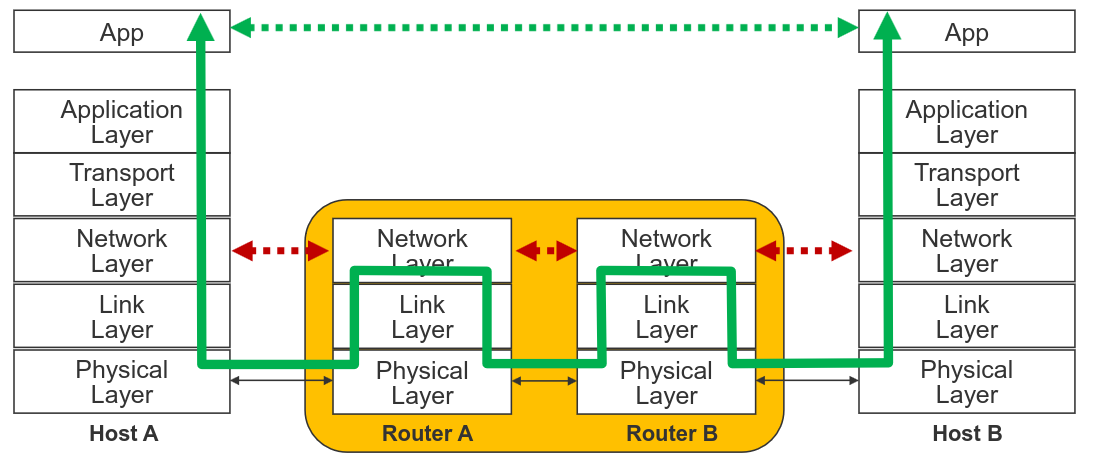
\includegraphics[scale=.3]{network}
\end{center}

\noindent There are two philosophies for \textbf{end-to-end connectivity}:
\begin{itemize}
	\item Connection-\textbf{less}: data is chunked and transferred as packets of variable length, with source and destination addresses in each one. Sending is made spontaneous without reservation. It's easy to implement but brings more challenges (wrong order of packets, delays, unreliability).
	\item Connection-\textbf{oriented}, with three phases:
	\begin{itemize}
		\item \textit{Connection establishment}
		\item \textit{Data transmission}: information exchange between the partners
		\item \textit{Connection termination}: release of the terminals and the channels
	\end{itemize}
	It's more complex to implement but brings reservation of capacity, flow control and no problem with sequence numbering.
\end{itemize}

\noindent Intermediate nodes need to \textbf{acquire} and \textbf{maintain} the \textbf{state} to establish paths, scope broadcasts and guarantee service quality. At the same time they need to handle \textbf{constraints}:
\begin{itemize}
	\item \textbf{Limited memory}: they cannot store an arbitrary amount of data
	\item \textbf{Limited throughput}: they cannot rely on an arbitrary amounts of control traffic to acquire the state
	\item \textbf{Limited computing capacity} and \textbf{speed}: they cannot compute arbitrary complex operations
\end{itemize}

\newpage
\subsection{Addressing}
Addresses are used to \textbf{identify} end hosts in multi-access networks and, in case of multi-address hosts, they help to select the right interface. They require:
\begin{itemize}
	\item \textbf{Compactness} of representation
	\item \textbf{Independence} from lower layers
	\item Built-in support for efficient and decentralized \textbf{path finding}
	\item \textbf{Uniqueness} within a network scope
\end{itemize}

\paragraph{Aggregation} Aggregation leads to much smaller intermediate states in intermediate nodes. Some example are:
\begin{itemize}
	\item \textbf{Geographical}: aggregate based on geographical area with a strict assignment policy
	\item \textbf{Hierarchical}: aggregate by organizations and sub-organizations, has a higher flexibility in assignment but may lead to less compression:
	\begin{itemize}
		\item \textit{Allocation}: initially a range of continuous addresses (determined by \textbf{prefix}) is given to an organization, which then can recursively delegate authority over parts of it. At the top the \textbf{Internet Assigned Numbers Authority} delegates to the \textbf{Regional Internet Registry} (AfriNIC, APNIC, ARIN, LACNIC and RIPE). They then delegate to \textbf{Local Internet Registry}, which are mostly ISP, enterprises or academic institution. They in the end assign IP to customers
		\item \textit{Assignment}: give an address to a host/interface
		\item \textit{Match}: longest common prefix match (match on prefix length), basically forward data to the output interface that shares more digits with the destination
	\end{itemize}
\end{itemize}

\paragraph{Challenges} The main challenges are:
\begin{itemize}
	\item \textbf{Security}: e.g. address spoofing when an attacker claims to own a network address of someone else since there is no global database
	\item \textbf{Efficiency}: effective aggregation requires careful address planning (keep large ranges, give unused addresses back)
	\item \textbf{Automation}: e.g. auto-configuration of address segment
\end{itemize}

\subsubsection{IPv4}
An IPv4 address is made of $4$ bytes divided in \textbf{network} part and \textbf{host} part. They can be:
\begin{itemize}
	\item \textbf{Public}: needs to be \textbf{unique}, typically one for each node
	\item \textbf{Private}: not unique and thus not globally routable.
\end{itemize}
\textit{Router} or \textit{gateways} usually have an IP address for each network they are linked to.
\begin{center}
	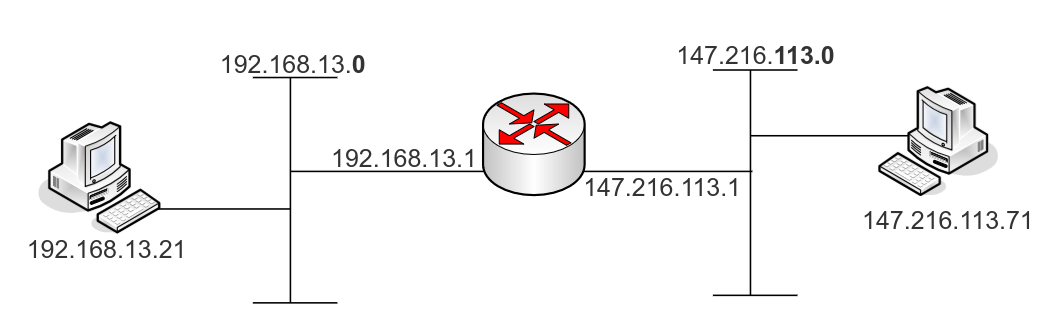
\includegraphics[scale=.3]{ipv4ex}
\end{center}

\paragraph{Classes}
\begin{wrapfigure}[5]{r}{5cm}
	\vspace{-0.5cm}
	\begin{center}
		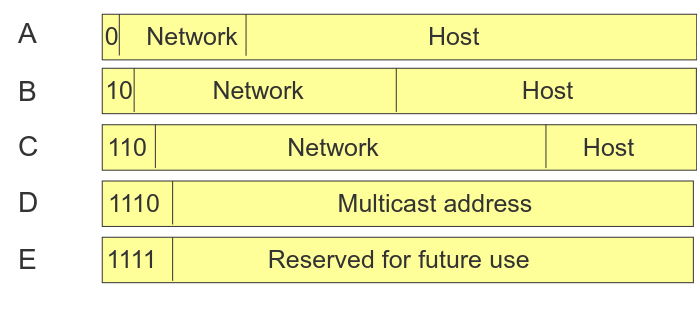
\includegraphics[width=5cm]{classes}
	\end{center}
\end{wrapfigure}
IP addresses are divided in five classes based on the first bits values. \\\\
Since nobody expected such an explosive growth of the internet, too many class A addresses were given away. Furthermore, class C networks are very small while class B are often too large.

\paragraph{Variable-Length Subnet Masking} To solve the problems of IP addresses, VLSM was introduced: static classes were replaced by network prefixes of any length.\\
Now an address is in the form $a.b.c.d/n$ where the first $n$ bits are the \textbf{network} identification and the remaining $32-n$ are the \textbf{host} identification. Another notation is the address and the explicit netmask in the form $u.x.y.z$.

\begin{note}
	VLSM is at the base of \textbf{Classless Inter-Domain Routing}.
\end{note}

\begin{definition}[Subnet]
	A subnet is a subset of addresses in a class A,B or C network. The principle is that some bits of the host addresses part are used to complement the network ID.
\end{definition}
All hosts on the same physical network use the same subnet mask. Combining IP address and subnet mask, a router determines to which subnet a packet must be sent.

\begin{center}
	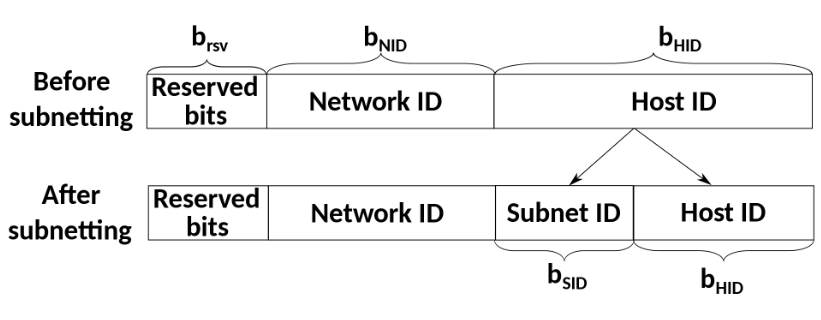
\includegraphics[scale=.3]{subnet}
\end{center}

\subsubsection{IPv6}
In 2011 IANA gives the last available blocks of IPv4 addresses. An extension was needed, hence the creation of IPv6: 128 bits divided in 8 couples of octets (8 bits).

\begin{note}
	IPv6 syntax allows to remove \textbf{leading zeros} in each one of the eight blocks and \textbf{replace} consecutive blocks of zeros with "::".
\end{note}

An IPv6 address is divided in three sections:
\begin{center}
	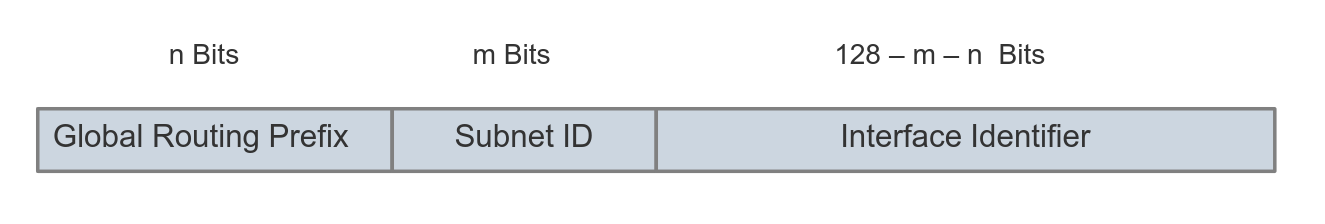
\includegraphics[scale=.3]{ipv6}
\end{center}
\begin{itemize}
	\item \textbf{Global Routing Prefix}: depends on RIR policy, for RIPE LIRs get /32 and ISPs get /48
	\item \textbf{Subnet Id}: assigned by network administrator
	\item \textbf{Interface identifier}: hash value identifying the NIC
\end{itemize}
\newpage
\noindent There are different types of addresses:
\begin{itemize}
	\item \textbf{Unicast}
	\begin{itemize}
		\item \textbf{Unique Local} $FC00::/7$
		\item \textbf{Link Local} $FE80::/10$
		\item \textit{IPv4-mapped} $::FF:0.0.0.0/96$
		\item \textit{Loopback} $::1/128$
		\item \textit{Unspecified} $::/128$
		\item \textbf{Global}: every other one
	\end{itemize}
	\item \textbf{Multicast} $FF00::/8$, it's an identifier for a group of interfaces. It has the following format:
	\begin{center}
		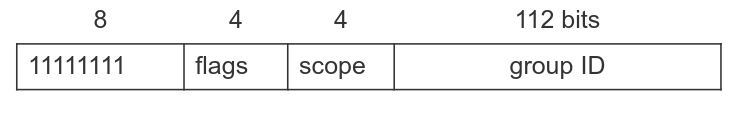
\includegraphics[scale=.3]{multicast}
	\end{center}
	\begin{itemize}
		\item \textbf{Flags}: 4 bits (0RPT) divided in:
		\begin{itemize}
			\item \textit{T}: if $1$, non permanently assigned (dynamically, on-demand), $0$ otherwise
			\item \textit{P}: multicast address assignment based on network prefix
			\item \textit{R}: embedding of the rendezvous point
		\end{itemize}
		\item \textbf{Scope}: defines the scope of the multicast
		\begin{table}[!h]
			\centering
			\begin{tabular}{c|c}
				\textbf{Value} & \textbf{Scope} \\
				\hline
				0 & Reserved \\
				1 & Interface-Local \\
				2 & Link-Local \\
				3 & Reserved \\
				4 & Admin-Local \\
				5 & Site-Local \\
				6, 7 & Unassigned \\
				8 & Organization-Local \\
				9-D & Unassigned \\
				E & Global scope \\
				F & Reserved
			\end{tabular}
		\end{table}
	\end{itemize}
	\item \textbf{Anycast}: chosen from unicast range and can be used to identify the router in a subnet, an organization or in a particular routing domain. It has the following format:
	\begin{center}
		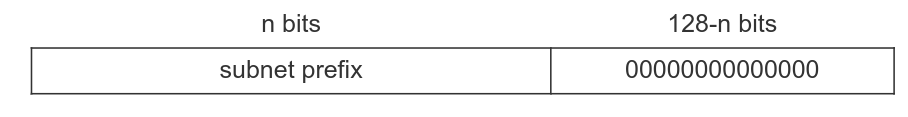
\includegraphics[scale=.3]{anycast}
	\end{center}
	\item \textbf{Broadcast}: dropped, use multicast
\end{itemize}

\newpage
\subsection{Internet Protocol}
Designing a protocol that serves the need for more than 40 years of technological development is really non-trivial since there is a continuous change of the upper- and lower-layer technologies.\\
Internet Protocol version 4 is the fundamental network layer protocol of the current Internet. The basic \textbf{properties} are:
\begin{itemize}
	\item \textbf{Transparent end-to-end communication} between hosts
	\item \textbf{Connectionless} and \textbf{packet-oriented}
	\item \textbf{Unreliable}, it provides a best-effort service
	\item \textbf{Hierarchical addressing}
	\item Support of \textbf{packet fragmentation}
\end{itemize}

\subsubsection{IPv4}
The IPv4 packet has the following format:
\begin{center}
	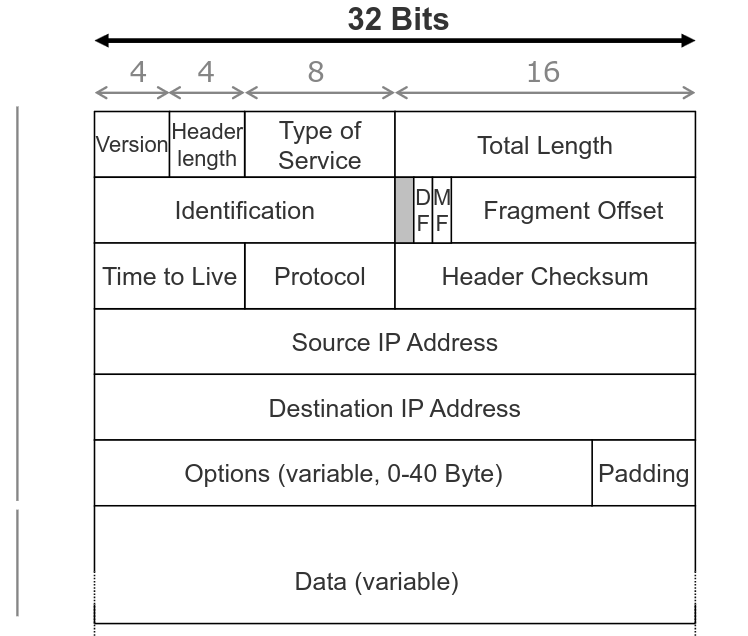
\includegraphics[scale=.3]{ipv4format}
\end{center}
\begin{itemize}
	\item \textbf{version}: either $4$ for IPv4 or $6$
	\item \textbf{length}: usually $20$ bytes but depends on the IP options
	\item \textbf{type of service}: allows different packets to be treated differently (e.g. low delay for voice, high bandwidth for video). Today it's used for \textbf{Differentiated Service Code Point} and \textbf{Explicit Congestion Notification}
	
	\paragraph{DSCP} This protocol is the introduction of \textbf{QoS} in IP network instead of best-effort. It uses a 6 bit flag and supports different types of services (e.g. video, voice). It defines various \textbf{Per-Hop Behaviors} that set the packet forwarding properties for a class of traffic:
	\begin{itemize}
		\item \textbf{Default}: best-effort traffic
		\item \textbf{Expedited}: loss-low, low-latency traffic
		\item \textbf{Assured}: assurance of delivery under prescribed conditions
		\item \textbf{Class Selector}: maintain backward compatibility with the old IP field
	\end{itemize}
	It introduces the principle of \textbf{traffic classification}, where each data packet is classified into one of a limited number of classes. Each router is then configured to differentiate traffic based on its class.
	
	\item \textbf{total length}: number of bytes of the entire packet, the maximum being $2^{16}-1$ bytes
	
	\paragraph{Fragmentation} Every link on the internet has a \textbf{Maximum Transmission Unit}, the number of bytes a link can carry as one unit. If the outgoing MTU is smaller than the total packet size, a router can \textbf{fragment} a packet, which are then recomposed at destination.
	
	\item \textbf{identification}: all fragments belonging to the same packet have this same value
	\item \textbf{More Fragments}: a single bit which indicates if this is the last fragment of a datagram $0$ or if further will follow $1$
	\item \textbf{Don't Fragment}: all router must forward packets up to a size of $576$ bytes, everything beyond that is optional. Larger packets with this bit set to $1$ might be discarded
	\item \textbf{fragment offset}: it's the position of a packet a fragment belongs to, counted in multiples of $8$ bytes
	\item \textbf{Time To Live}: it's used to limit packet travel time and identify and mitigate loops. Its value is decremented by $1$ at each router it passes and it's discarded when it reaches $0$
	\item \textbf{protocol}: identifies the higher-level protocol, such as TCP or UDP
	\item \textbf{header checksum}: it's the sum of all $16$ bits words in the header
	\item \textbf{source IP address}
	\item \textbf{destination IP address}
	\item \textbf{options}: were initially put to provide additional flexibility but now for security reasons are often deactivated since they could reveal information
\end{itemize}

\subsubsection{IPv6}
IPv6 was implemented first of all to have more addresses. But that was not the only reason:
\begin{itemize}
	\item Simpler \textbf{addressing} and \textbf{routing}
	\item Simpler \textbf{protocol architecture}: slim fixed header, optional extensions, format framework for header classes, no header checksum (done in other layers) and no fragmentation
	\item Simpler \textbf{administration}: auto-configuration of interfaces without DHCPv6 and renumbering via prefix change
	\item Additional \textbf{security}, improved multicast, anycast, \textbf{QoS}, support of \textbf{Jumbograms}
\end{itemize}

\paragraph{History} IP next generation work began in the early 90s: in 1992 there were several proposal for the development of IP. After several merges in 1993 \textbf{Simple Internet Protocol Plus} and \textbf{Common Architecture for the Internet} were created. In 1994, SIPP was chosen.\\
In 1995 the IPv6 specification rolled out and in 1999 user addresses were available. \\
In May 2007 ARIN advises the beginning of IPv6 migration and in 2012 there is the world launch.

\paragraph{Packet} The packet is formatted as follows:
\begin{center}
	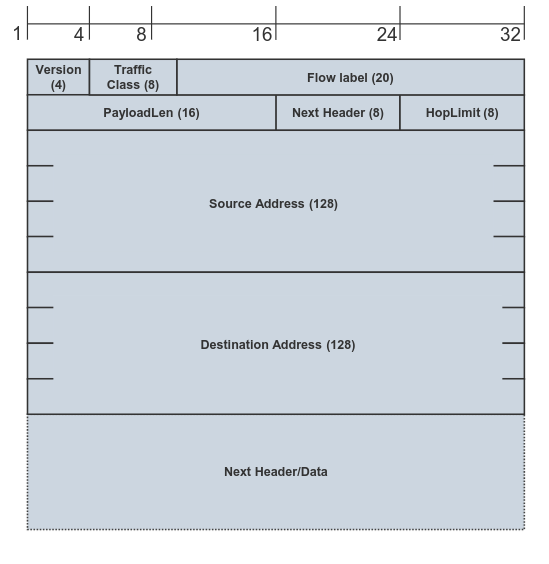
\includegraphics[scale=.28]{ipv6format}
\end{center}

\begin{itemize}
	\item \textbf{version}: IP version number
	\item \textbf{traffic class}: classifying packets
	\item \textbf{flow label}: virtual connection with certain characteristics or requirements
	\item \textbf{payloadLen}: packet length after the 40 bytes header
	\item \textbf{nextHeader}: indicates the type of the following extension header or the transport header
	\item \textbf{hopLimit}: decremented by one at each hop, if zero discarded
	\item \textbf{source address}
	\item \textbf{destination address}, not necessary if there is an optional routing header
	\item \textbf{next header/data}, if an extension header is specified, it follows after the main header, otherwise the data are following
\end{itemize}

\paragraph{Comparison} The IPv6 header is longer than the IPv4 but it's only because of the longer addresses. Otherwise, it's better sorted and thus \textbf{faster} to process by routers.\\
\textbf{Fragmentation} was removed, among with checksum and header length, to leave the problem to the end host and simplify the handling.

\paragraph{Extension headers} They extend basic IPv6 functionalities. Each header may either reference another extension or the data. The main extensions are:
\begin{itemize}
	\item \textbf{Routing}: definition of a full or partly specified route (deprecated since 2007)
	\item \textbf{Fragmentation}: same as IPv4 but now only the source can fragment and if a router finds a packet that's too big, an error is sent back
	\item \textbf{Authentication}: security information, authentication of the sender
	\item \textbf{Encapsulation}: tunneling e.g. for encrypted data
	\item \textbf{Hop-by-Hop options}: dedicated options to be processed by every router and host, at the moment only the Jumbogram implementation is supported
	\item \textbf{Destination options}: additional information for the destination
\end{itemize}

\paragraph{Options} For maximum flexibility, options are possible in headers. They have no length limit and are encoded as \textbf{Type-Length-Value}:
\begin{center}
	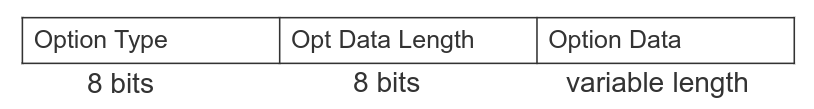
\includegraphics[scale=.3]{tlv}
\end{center}
The \textbf{Option Type} defines also:
\begin{center}
	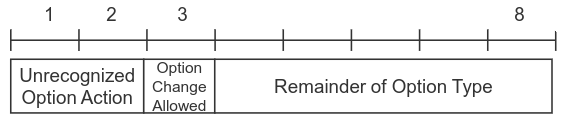
\includegraphics[scale=.3]{options}
\end{center}
\begin{itemize}
	\item \textbf{Unrecognized Option Action}: the action that must be taken if a node does not recognize the Option Type
	\begin{itemize}
		\item $00$: skip this option and continue with the rest
		\item $01$: discard the packet
		\item $10$: discard the packet and ICMP the source with \textit{unicast} and \textit{multicast}
		\item $11$: discard the packet and ICMP the source with \textit{unicast}
	\end{itemize}
	\item \textbf{Option Change Allowed}: indicates whether or not the \textbf{Option Data} can be modified while the datagram is en route
\end{itemize}

\begin{observation}[Length]
	IPv6 requires a minimum \textbf{MTU} of 1280 bytes. Links which cannot convey such big packets have to apply link-specific fragmentation and assembly at a layer below IPv6.
\end{observation}

\paragraph{Path MTU} It's the minimum link MTU of all the links in a path between a source node and a destination node. The originating node assumes that the PMTU is the MTU of the first hop. A \textbf{trial packet} of that size is sent out. If any link is unable to handle it, an ICMPv6 Packet \textbf{Too Big} is sent back and the originating node tries again with a smaller MTU.

\subsubsection{Migration}
IPv6 cannot be introduced overnight: for some time both variants will coexist. An \textbf{incremental deployment} is needed, which includes:
\begin{itemize}
	\item \textbf{Porting}: making applications IPv6 ready, which means using a new API
	\item \textbf{Migration}: done step by step through different techniques
	\begin{itemize}
		\item \textbf{Dual stack}: allowing the coexistence of both versions on the same device and subnet. The application chooses which one to use. It can continue indefinitely but means an increased use of IPv4 NAT.
		\begin{center}
			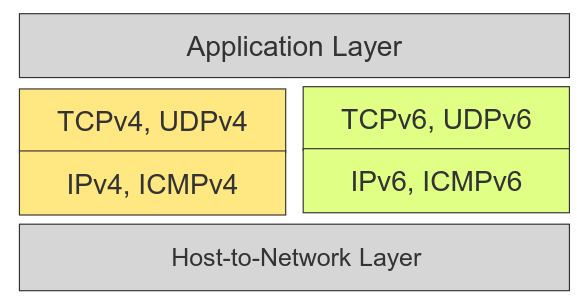
\includegraphics[scale=.2]{dualstack}
		\end{center}
		One of the main protocols is \textbf{Dual Stack Lite}: there is no IPv4 in the public internet, just in the private networks. IPv4 runs then over IPv6 and many customers can share a single globally unique IPv4 address.
		\item \textbf{Tunneling}: connecting IPv6 regions over IPv4 regions. Routers encapsulates incoming IPv6 packets into a new IPv4 one with destination address of the next router also supporting IPv6. There is more \textbf{overhead} but no data loss.The main techniques are:
		\begin{itemize}
			\item \textbf{6-over-4}: IPv6 islands in an IPv4 world with an IPv6 backbone. The end-user site network stuff must choose an IPv6 Internet Service to tunnel to or peer with other islands
			\item \textbf{6-to-4}: isolated IPv6 islands in an IPv4 world. It allows the islands to automatically interconnect, defining \textbf{point-to-multipoint tunnels} and assigning an IPv6 prefix to each IPv4 address (DNS will return both). Then the nearest router identifies 6to4 packet based on a special IPv6 prefix and encapsulates it in IPv4
		\end{itemize}
		\item \textbf{Protocol Translator} (NAT): let IPv6 devices speak to IPv4 ones
	\end{itemize}
\end{itemize}

\newpage
\subsection{Assignment and mapping}
\subsubsection{ARP}
The \textbf{Address Resolution Protocol} discovers the MAC addresses associated with an IP address, which is needed for the lower layers that do not understand IP.\\
Each host stores known IP and MAC addresses in a table: the \textbf{ARP cache}. The entries become invalid after a certain amount of time, to avoid mistakes. The entries are inserted through ARP \textbf{requests} (broadcasts) and \textbf{responses}. \\
To optimize the process, each computer occasionally sends an ARP request to it's own IP address. On some systems a host periodically sends out requests for each entry.\\
The packet format is designed to be used with various network and link layers by specifying the length:
\begin{center}
	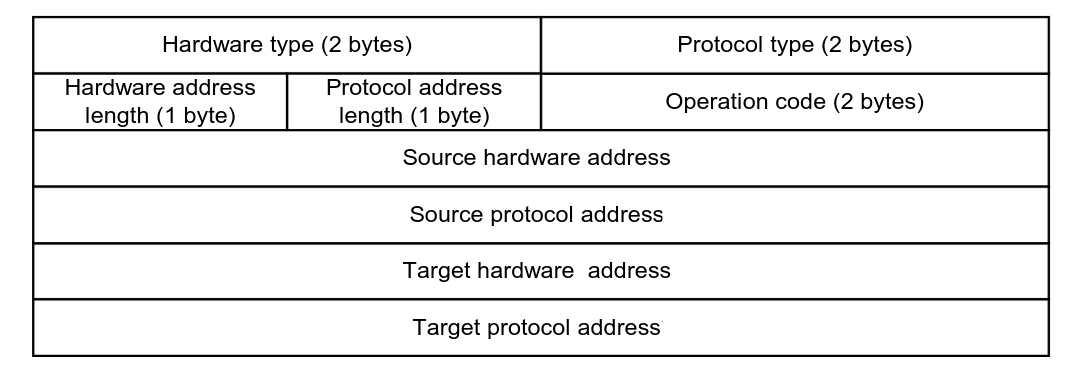
\includegraphics[scale=.3]{arp}
\end{center}

\paragraph{Risks} Since an ARP request-response is \textbf{stateless} and \textbf{not authenticated}, the ARP cache is updated every time it receives a reply, even if it didn't send out one. This creates risks for:
\begin{itemize}
	\item \textbf{Spoofing}: a rogue machine can spoof other machines by replying with wrong data
	\item \textbf{Cache poisoning}: a rogue machine can poison an ARP cache by sending forged ARP replies
\end{itemize}

\subsubsection{RARP}
The \textbf{Reverse} Address Resolution Protocol a computer can ask it's own IP address by sending out his MAC address. A RARP server then replies with the IP. Deprecated.

\subsubsection{DHCP}
\begin{wrapfigure}[10]{r}{8cm}
	\vspace{-1.5cm}
	\begin{center}
		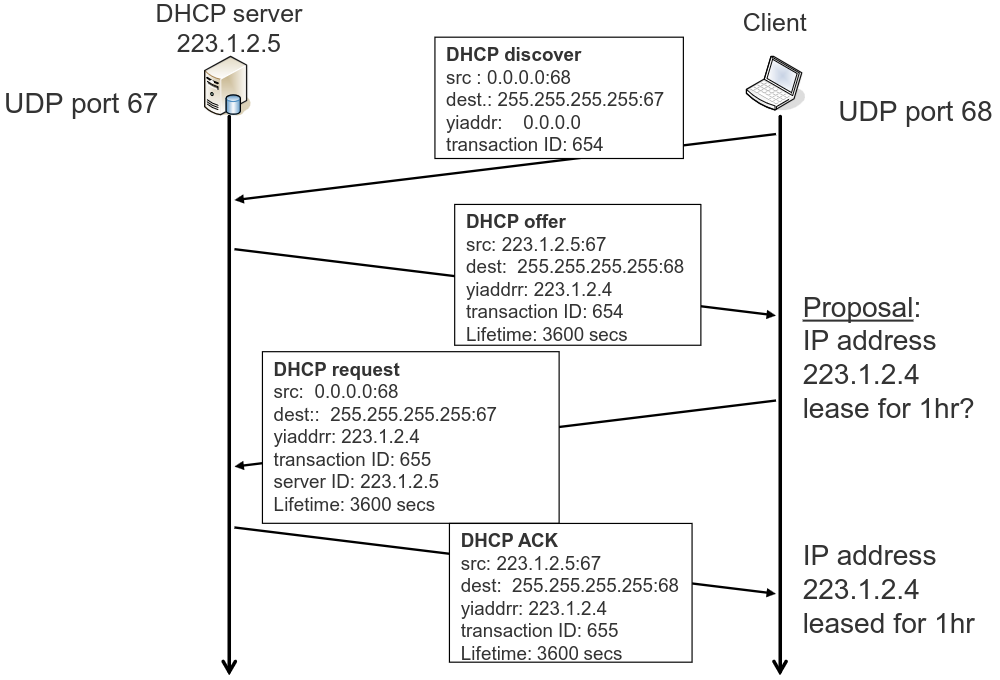
\includegraphics[width=7cm]{dhcp}
	\end{center}
\end{wrapfigure}
Since RARP requests are not passed on by routers, the computer sends out a DHCP packet. In each subnet there is also a \textbf{DHCP Relay Agent} which passes those messages to the DHCP server.\\
Furthermore, to communicate globally you need more than the IP address (subnet mask, defaul router, DNS server) and those are configured by the DHCP.\\
DHCP works in three phases:
\begin{itemize}
	\item \textbf{Service discovery}: the host does a \textbf{DHCP Discover} (broadcast), where he states his MAC address and asks for an IP one. The server then answers with a \textbf{DHCP Offer} (unicast) where he offers the IP address and other configurations (DHCPINFORM).
	\item \textbf{IP Address Assignment}: the host sends out a \textbf{DHCP Request} (broadcast) stating his MAC address and the IP address that he wants to use. The server sends out a \textbf{DHCP Ack} (unicast) to accept that (or NACK to deny).
	\item \textbf{Address release}: IP addresses may be permanently assigned or leased for a limited period of time. After the lease expiration you need to explicitly renew the lease or relinquish the address (\textbf{DHCPRELEASE})
\end{itemize}

The DHCP packet format was mostly inherited from a previous protocol (BOOTP) and its the following:
\begin{center}
	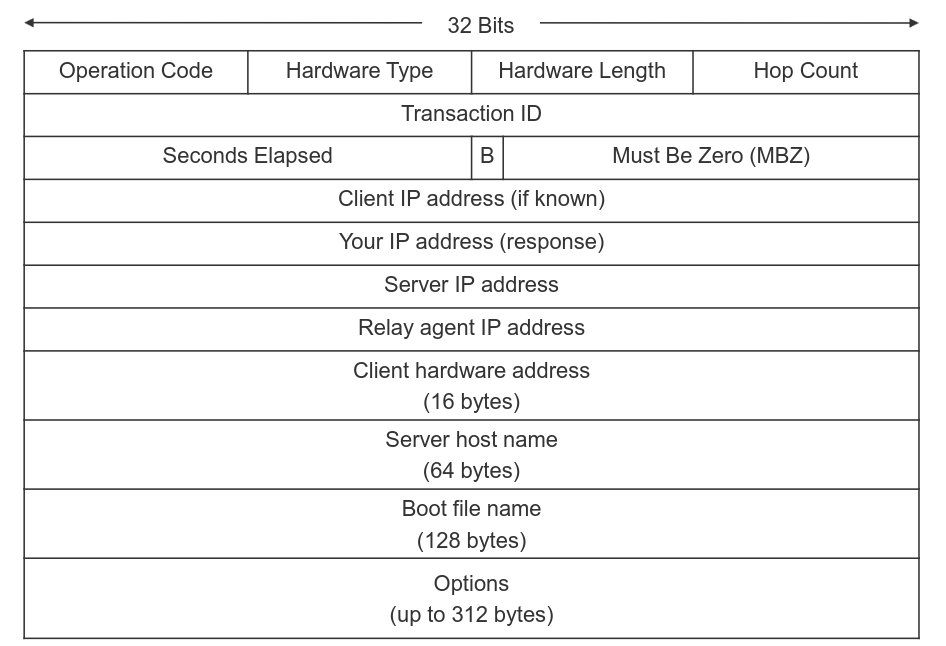
\includegraphics[scale=.3]{dhcpformat}
\end{center}

\begin{note}
	DHCP uses UDP and therefore is \textbf{unreliable}.
\end{note}

\subsubsection{NDP}
In IPv6 instead of ARP, \textbf{Network Discovery Protocol} is used. This protocol is also used for:
\begin{itemize}
	\item \textbf{Neighbor Unreachability Detection}
	\item IPv6 \textbf{address autoconfiguration}
	\item \textbf{Router discovery}
	\item \textbf{On-link prefix discovery}
	\item \textbf{Next-hop determination}
	\item \textbf{Link parameter discovery}, e.g. MTU
	\item \textbf{Redirect}: indicate better next-hop
	\item \textbf{Duplicate Address Detection}
\end{itemize}

\noindent The packet format is a classic ICMPv6 one:
\begin{center}
	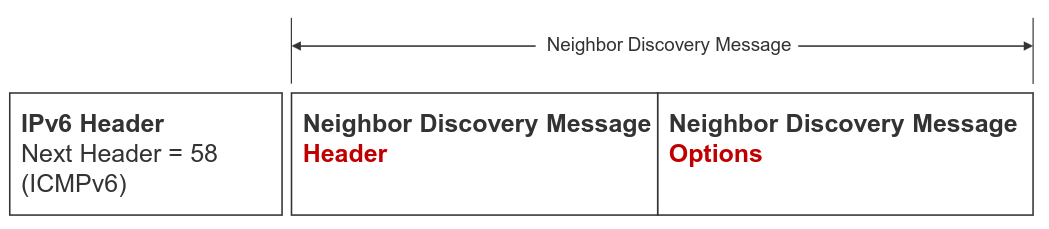
\includegraphics[scale=.3]{ndp}
\end{center}
The possible operations are, compared to IPv4:
\begin{table}[!h]
	\centering
	\begin{tabular}{|c|c|}
		\hline
		\textbf{IPv6} & \textbf{IPv4} \\
		\hline
		\textit{Neighbor Solicitation} & ARP Request \\
		\hline
		\textit{Neighbor Advertisement} & ARP Reply \\
		\hline
		\textit{Neighbor Cache} & ARP Cache \\
		\hline
		\textit{Router Solicitation}& Router Solicitation \\
		\hline
		\textit{Router Advertisement} & Router Advertisement \\
		\hline
		\textit{Redirect Message} & Redirect Message\\
		\hline
	\end{tabular}
\end{table}

\begin{note}
	One advantage of using NDP is that it's a pure network protocol contrary to ARP, meaning that one can also apply network layer security mechanisms solving problems like spoofing.
\end{note}

\subsubsection{SLAAC}
\textbf{State-Less Address Auto-Configuration} is the IPv6 stateless equivalent for DHCP. It's divided in three phases:
\begin{enumerate}
	\item \textbf{Acquire Link Local} IPv6 address: generate a tentative link-local based on the MAC address, used \textbf{Duplicate Address Detection} (send a \textit{Neighbor Solicitation} to that address): if the address exists, fail and go to manual, otherwise if there is no response, convert the \textbf{Extended Unique Identifier} 48 bits MAC into a EUI 64 bit dynamically assigned host identifier:
	\begin{enumerate}
		\item Leftmost 24 bit of the MAC form the leftmost 24 bits of the EUI-64
		\item Rightmost 24 bit of the MAC form the rightmost 24 bits of the EUI-64
		\item Insert the constant $FFFE$ in the middle
		\item Tweak left-most bit 7 from zero to one
		\item Prepend $FE80::$
	\end{enumerate}
	\item \textbf{Contact router}: once the link-local address is assigned to the interface, the node sends out a \textbf{router solicitation} to the well-known address $FF02::1$ (All Routers) and the router responds with a \textbf{Router Advertisement}
	\item \textbf{Configure Global IPv6 Addresses}: process the \textit{router advertisement} message that has been received, which includes the network ID prefix and two flags:
	\begin{itemize}
		\item \textbf{Managed Address Configuration}: if $1$, stop and do stateful configuration, otherwise assign the global IP Global IP:Host ID/64 and check the other flag
		\item \textbf{Other Stateful Configuration}: if $0$, stop, otherwise use stateful configuration for other information such as name server
	\end{itemize}
\end{enumerate}

\subsection{Diagnostic}
\subsubsection{ICMP}
Internet Control Message Protocol is a \textbf{control} protocol of layer 3. It has two use cases:
\begin{itemize}
	\item If a router cannot forward a packet, the source can be informed about it via an ICMP message
	\item \textbf{Ping} uses ICMP request and reply to check if host is online
\end{itemize}
The packet format is the following:
\begin{center}
	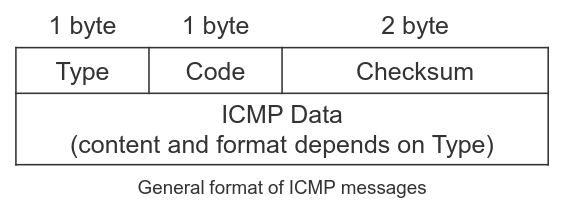
\includegraphics[scale=.3]{icmp}
\end{center}
\begin{itemize}
	\item \textbf{Type}: purpose of the message, 40+ types are defined and 41-255 are reserved for future use. The most important are:
	\begin{itemize}
		\item $0$: \textit{destination unreachable}
		\item $3$: \textit{echo} request and reply
		\item $4$: \textit{Source Quench} (choke packet)
		\item $11$: TTL reached 0, packet discarded
		\item $12$: parameter problem on datagram
		\item $15/16$: information request and reply
		\item $30$: \textit{traceroute}
	\end{itemize}
	\item \textbf{Code}: additional information about the condition
	\item \textbf{Checksum}
	\item \textbf{Data}: there are mainly two message categories
	\begin{itemize}
		\item \textbf{Error}: to report an event. These messages don't have a response and include the IP header that generated the error
		\item \textbf{Queries}: to get some information from a node, they have a matching response
	\end{itemize}
\end{itemize}

\paragraph{IPv6} The packet format is the same for IPv6 but it's used for way more purposes, such as:
\begin{itemize}
	\item Automatic address configuration (NDP/SLAAC)
	\item Automatic MTU Path discovery
	\item PacketTooBig is sent to source (IPv6 has no fragmentation)
	\item IGMP
	\item Detect malfunctioning router and inactive hosts
	\item Routing (RPL)
\end{itemize}

\subsection{Network Address Translation}
\begin{wrapfigure}[5]{r}{5cm}
	\vspace{-0.5cm}
	\begin{center}
		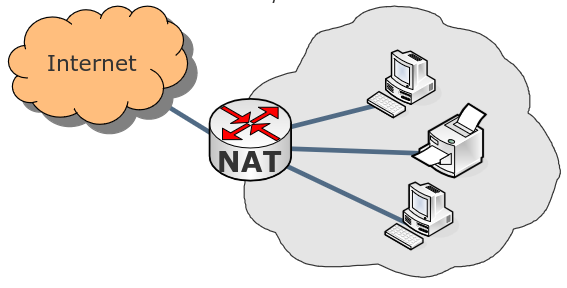
\includegraphics[width=5cm]{nat}
	\end{center}
\end{wrapfigure}
Each device needs an IP address, but they are scarce. Hence a well-known block of IP addresses were reserved for site-local use:
\begin{itemize}
	\item Class A: $10.0.0.0$ to $10.255.255.255$
	\item Class B: $172.16.0.0$ to $172.16.255.255$
	\item Class B: $192.168.0.0$ to $192.168.255.255$
\end{itemize}
This allows for the reuse of the same private address within a different site \textbf{scalability} but introduces the need of sharing a public IP address through NAT.

\begin{observation}[Security]
	While some may argue that NAT hides the internal structure of a network and avoids exposing hosts, it doesn't actually improves security (e.g. doesn't prevent DDOS), it's only an excuse to prevent deployment of clean networks.
\end{observation}

\subsubsection{Static}
Static NAT hides the structure of the network using one public IP address per private IP address, mapping them permanently. This means that we need as many public addresses as the private ones.\\
\textbf{Temporary mapping} can be done, managing a pool of public addresses and assigning them dynamically when a request is sent out, but during peak traffic the number of public IPs used is almost the same as the private ones.
\begin{center}
	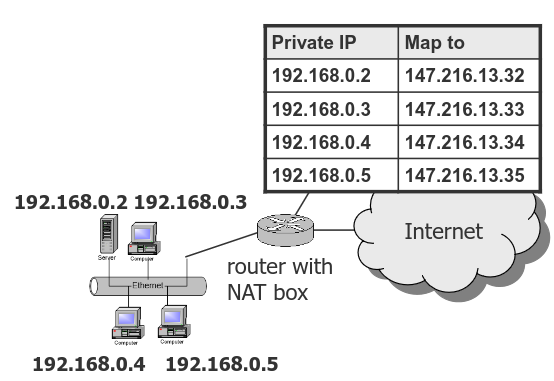
\includegraphics[scale=.3]{snat}
\end{center}

\subsubsection{One-to-Many}
Also known as \textbf{masquerading}, translates several local addresses into the same public address. Demultiplexing is now necessary and it's done through \textbf{Network Address Port Translation}: when a packet is sent out, the NAT box saves the local IP and port and maps them to a global port and IP, together with the destination IP and port. When the message comes back, it's remapped to the original address.
\begin{center}
	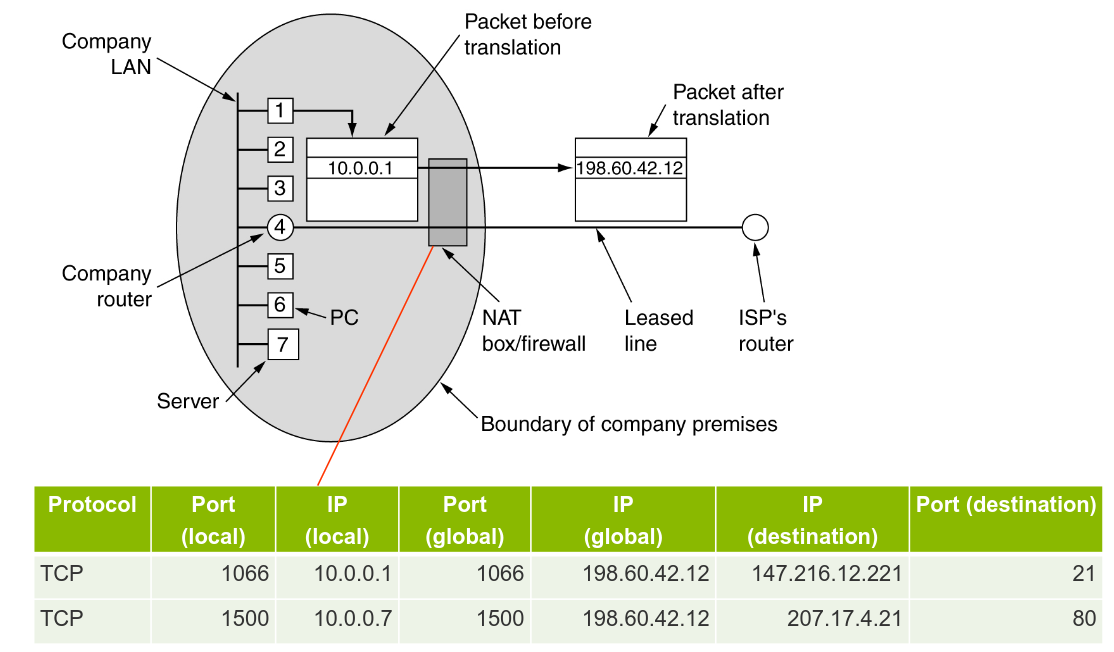
\includegraphics[scale=.3]{napt}
\end{center}
The main \textbf{problems} with this NAT technique arise when the message arrives from the outside. Some static information need to be stored, such as "forward each request with port 80 to host x". Still, problems remains (e.g. instant messaging).

\subsubsection{Carrier Grade}
Also known as \textbf{Large Scale} NAT, it uses a NAT box for a large number of customers (e.g. a street) to further mitigate address exhaustion. It breaks end-to-hand principle and it's difficult to use well-known ports.

\subsubsection{NAT64}
It's a mechanism to connect IPv6 hosts to IPv4 servers: the client embeds an IPv4 address and then the NAT changes the IP headers, mapping IPv6 to IPv4.

\subsubsection{Issues}
The main issues with NAT are:
\begin{itemize}
	\item \textbf{Header checksum}: changing IP addresses or port numbers on the fly requires also the recalculation of the checksum
	\item \textbf{Fragmentation}: since transport ports are part of the first fragment and packets may be delivered out of order, you need per fragment states in the NAT box
	\item \textbf{Encryption}: you cannot change fields values that are encrypted
	\item \textbf{Protocol-specific} issues above network layer, e.g. with DNS you will need static NAT mappings to match DNS entries
\end{itemize}
Overall, while NAT saved the internet, it killed the principle of \textbf{end-to-end} communication being initiated by one side.

\newpage
\subsection{Routing}
A \textbf{router} (any host can be) accepts packets from third parties and forwards them. Router behavior coordinates within the network.\\
Inside a router there are:
\begin{itemize}
	\item \textbf{Routing table}: contains the paths selected by the router for the forwarding table
	\begin{itemize}
		\item \textit{Destination network}
		\item \textit{Network mask}
		\item \textit{Meta information}, e.g. path length
		\item \textit{Next hop}
	\end{itemize}
	\item \textbf{Forwarding table}: contains the destination network to which the router sends the packet
\end{itemize}
To find the entry that overlaps most with a destination IP address, \textbf{Longest Common Prefix Match} is used: the bit of the destination address are compared to the network mask of each entry and the one with the longest match is chosen. If no entry fits, the \textbf{default route} is chosen.\\\\
Path selection also depends on the \textbf{application scenario}:
\begin{itemize}
	\item \textbf{Intra}-domain: when routers belong to the same administrative domain they  all have the same understanding what a best path is
	\item \textbf{Inter}-domain: when routers belong to different domains, path selection with individual policies is needed
\end{itemize}

\begin{note}
	Let's keep in mind two \textbf{prerequisites}:
	\begin{itemize}
		\item Each node must have at least one \textbf{unique} IP address (may have multiple)
		\item The \textbf{scope of validity} of the IP address should be appropriate (not link-local or private in case of global communication)
	\end{itemize}
\end{note}

\subsubsection{Router vs Forwarding}
\begin{definition}[Forwarding]
	A \textbf{local} process, which runs on a single machine, and moves incoming packets from input interface to appropriate output interface, towards their destination.
\end{definition}

\begin{definition}[Routing]
	A \textbf{distributed} process, which requires the cooperation of several devices (routers) in the network. Monitoring and exchanging enough network topology information between them to allow correct \textit{forwarding} decisions on each one.
\end{definition}

\begin{definition}[Routing table]
	The \textbf{raw topology} information acquired by routing. It's shape and format depends on the used technique, sometimes it may not even exist.
\end{definition}

\begin{definition}[Forwarding table]
	The \textbf{final product} of the routing process: it's derived from the raw topology information acquired by the routing scheme.
\end{definition}

\paragraph{Forwarding scheme} Moves packets from one input interface to appropriate output interface, according to what is currently in the forwarding table. The requirements are:
\begin{itemize}
	\item \textbf{Scalability} in therms of \textbf{IO transfer speed}
	\item \textbf{Fast table lookup}:
	\begin{itemize}
		\item \textbf{One-dimensional}, depends only on the destination, paths from different sources coincide when they overlap
		\item \textbf{Two-dimensional}, depends on the source and the destination, the paths may differ
	\end{itemize}
	Furthermore, the match can be done:
	\begin{itemize}
		\item \textbf{Longest Prefix Match}
		\item \textbf{Exact Label Match}
	\end{itemize}
	\item \textbf{Efficient} and sophisticated \textbf{data structures}
\end{itemize}
\newpage
\noindent Forwarding schemes can be:
\begin{itemize}
	\item \textbf{Deterministic}: decision based only on key lookup
	\item \textbf{Probabilistic}: decision based on key lookup and/or \textbf{random}
\end{itemize}
So, in the end, routing is the \textbf{control-plane} that computes, populates and maintains the forwarding table, while forwarding describes how the data flows, the \textbf{data-plane}.

\begin{table}[!h]
	\centering
	\begin{tabular}{c|c|c}
		& \textbf{forwarding} & \textbf{routing} \\
		\hline 
		\textbf{goal} & direct packet to outgoing link & computes paths packet will follow \\
		\textbf{scope} & local & network-wide \\
		\textbf{timescale}  & nanoseconds & milliseconds
	\end{tabular}
\end{table}

\subsubsection{Routing schemes}
A routing scheme \textbf{monitors} and \textbf{exchanges} \textbf{network topology information} between routers to allow correct forwarding decisions on each one of them. The requirements are:
\begin{itemize}
	\item \textbf{Scalability} in terms of \textbf{network-wide convergence speed}
	\item \textbf{Small control overhead} in terms of memory, throughput and CPU
	\item \textbf{Fault tolerance} to guarantee maximum availability
	\item \textbf{Loop-freedom}
	\item \textbf{Flexibility} to accommodate different path requirements for different applications
\end{itemize}
\paragraph{Static vs Dynamic}
\begin{itemize}
	\item \textbf{Static}: static forwarding tables are used, hence no reaction to changes in the network. It's \textbf{simple} and \textbf{stable} but in case of link or router breakdown, catastrophic
	\item \textbf{Dynamic}: routing tracks the network continuously and the forwarding tables are updated upon topology changes. It's \textbf{fault-tolerant} and more \textbf{reliable} but more \textbf{complex} and with more \textbf{overhead}
\end{itemize}

\paragraph{Source vs Hop-by-Hop}
\begin{itemize}
	\item \textbf{Source}: the path is determined by the source node and the whole path is included in the packet. In this scheme the routers do not need state but there is no fault tolerance if a downstream router or a link breaks
	\begin{center}
		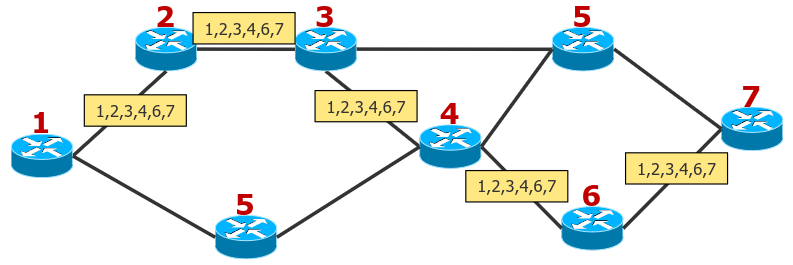
\includegraphics[scale=.4]{source}
	\end{center}
	\item \textbf{Hop-by-Hop}: the path is determined by each intermediate router, allowing for fault-tolerance but introducing state
\end{itemize}

\newpage
\paragraph{Packet vs Virtual Circuits}
\begin{center}
	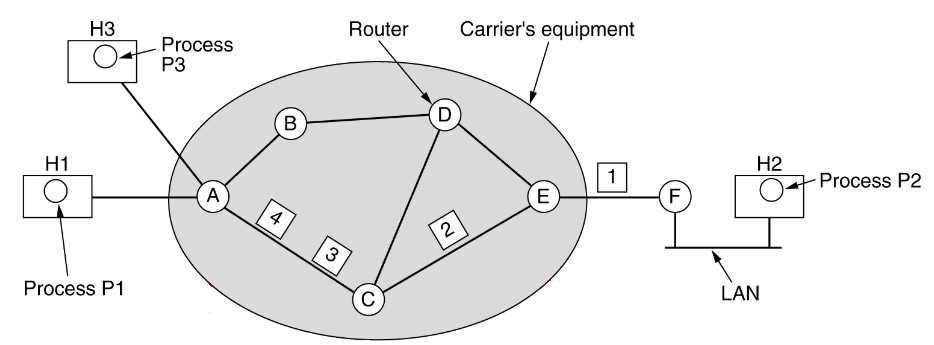
\includegraphics[scale=.35]{pvc}
\end{center}
\begin{itemize}
	\item \textbf{Packet}: \textbf{connectionless}, forwarding with the longest \textit{prefix match} at each hop
	\begin{center}
		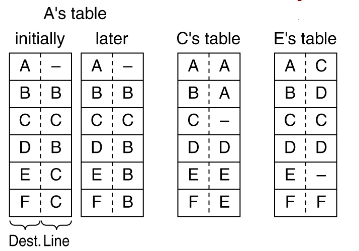
\includegraphics[scale=.4]{packetrouting}
	\end{center}
	\item \textbf{Circuit switching}: \textbf{connection-oriented}, forwarding with exact match at each hop
	\begin{center}
		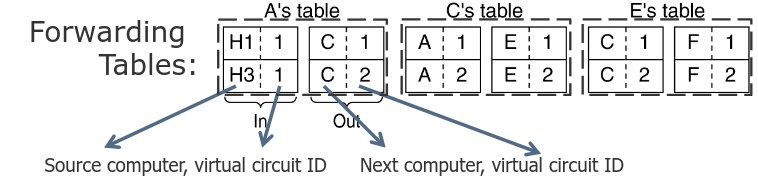
\includegraphics[scale=.4]{vc}
	\end{center}
\end{itemize}

\begin{table}[!h]
	\centering
	\begin{tabular}{c|p{4cm}|p{4cm}}
		& \textbf{Packet} & \textbf{Circuit Switching} \\
		\hline
		\textit{Circuit setup} & Not needed & Required \\
		\hline
		\textit{Addressing} & Each packet contains the full source and destination address & Each packet contains a short VC label \\
		\hline
		\textit{Forwarding} & Longest prefix match & Exact label match \\
		\hline
		\textit{Routing} & Dynamic routing & Static routing \\
		\hline
		\textit{Router failure impact} & None, except for packet loss during the crash & All VCs that passed through the failed router are terminated \\
		\hline
		\textit{QoS} & Difficult & Easy if enough resources can be allocated in advance \\
		\hline
		\textit{Congestion control} & Difficult & Easy if enough resources can be allocated in advance 
	\end{tabular}
\end{table}

\paragraph{Reactive vs  Proactive}
\begin{itemize}
	\item \textbf{Reactive}: a path is discovered and maintained only when applications ask for it, less control overhead but path exploration delays, hence needs user data buffering
	\item \textbf{Proactive}: al possible path are discovered and maintained a priori, avoiding delays and buffering but introducing control overhead
\end{itemize}

\paragraph{Hierarchical vs Flat}
\begin{itemize}
	\item \textbf{Hierarchical}: definition of separate virtual regions in the network, hierarchically organized in a simil tree structure, with a central region as root. Less state required, as routers only need to know about their region, but may lead to worse paths since there is partial topology knowledge.
	\item \textbf{Flat}: all routers are part of the same region, having more state and overhead but being able to reach the best paths due to full topology knowledge
\end{itemize}

\subsubsection{Basic concepts}
\paragraph{Flooding}
\begin{wrapfigure}[7]{r}{5cm}
	\vspace{-2cm}
	\begin{center}
		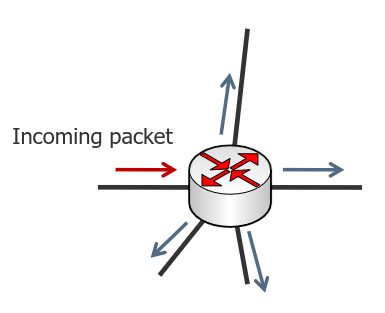
\includegraphics[width=5cm]{flooding}
	\end{center}
\end{wrapfigure}
Flooding means that each router \textbf{repeats} a received packet over all its interfaces, except for the source one. Each packet will reach all routers, meaning very \textbf{robust} in case of failure. At the same time there are several problems: \textbf{privacy}, \textbf{goodput decrease} and there must be a \textbf{loop detection}.

\begin{note}
	In a \textbf{wireless} context, flooding means repeating packets on the interface they were received from.
\end{note}

In conclusion, flooding does not scale well but it's used by some routing algorithms (OSPF) and can be used as a benchmark.

\paragraph{Metrics} Metrics compares the available paths discovered by routing to find the most favorable one. This depends on different criteria:
\begin{itemize}
	\item \textbf{Response time}
	\item \textbf{Throughput capacity}
	\item Least number of \textbf{intermediate devices}
	\item \textbf{Avoidance} of local \textbf{overload}
	\item \textbf{Security} requirements
\end{itemize}
Routing algorithms generally take as input a \textbf{cost} per \textit{link}. Unless specified otherwise, all links have the same cost and it may be updated by external mechanisms. The algorithms then find the available paths with the smallest \textbf{end-to-end cost}, which depends on three main metrics:
\begin{itemize}
	\item \textbf{Additive}: add cost of each link on the path, e.g. delay
	\item \textbf{Multiplicative}: multiply cost of each link on the path, e.g. packet delivery ratio
	\item \textbf{Concave}: minimum cost of all links on the path, e.g. throughput
\end{itemize}
\begin{note}
	The default metric, in case of equal cost, is the \textbf{hop-count}.
\end{note}

Determining the optimal path may be difficult because topology and information are never instantly available. Moreover, some metrics leads to \textbf{NP-complete} computations and \textbf{conflicts} between fairness and optimum can arise.

\newpage
\paragraph{Graphs} A computer network can be abstracted as a weighted graph where:
\begin{itemize}
	\item \textbf{Vertex} is a router
	\item \textbf{Edge} is a link
	\item \textbf{Weight} is the cost of the link
\end{itemize}
Routing algorithms must discover and maintain a \textbf{partial}, but \textbf{sufficient} view of the topology to make paths available, from anywhere to everywhere.
\begin{figure}[!h]
	\hfil
	\subfigure[Full topology]{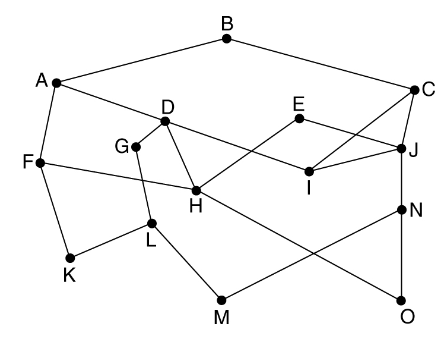
\includegraphics[scale=0.4]{fulltop}}
	\hfil
	\subfigure[Partial topology]{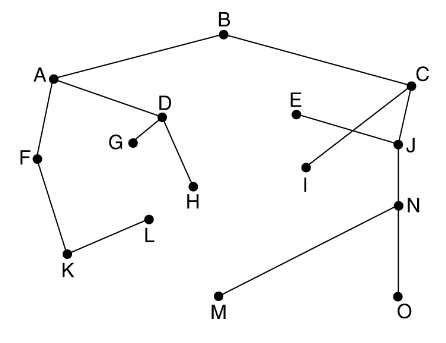
\includegraphics[scale=0.4]{parttop}}
\end{figure}

\subsubsection{Algorithms}
Routing algorithms are divided as follows:
\begin{center}
	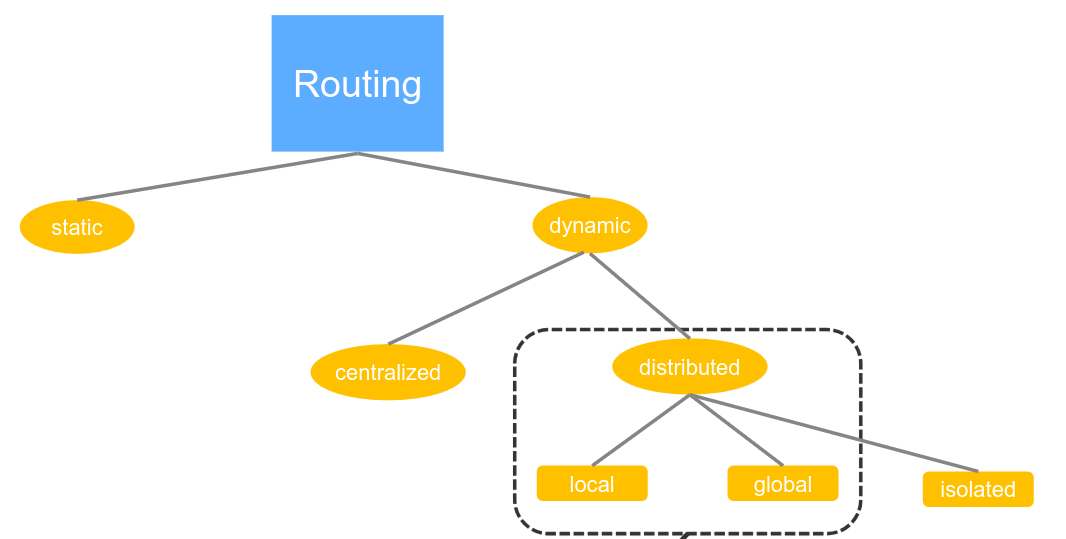
\includegraphics[scale=.4]{taxonomy}
\end{center}

\paragraph{Distance Vector Routing} E.g. \textbf{RIP}. The main principle is that \textbf{global information} is exchanged \textbf{locally}:
\begin{enumerate}
	\item Each router periodically sends out a list of destinations it can reach including the costs to each one
	\item If a router received that list and updates its own forwarding table with new paths or better ones
	\item The algorithm converges towards a state where the forwarding table of each router indicates the least cost path to each possible destination
\end{enumerate}
\newpage
\noindent This corresponds to the \textbf{Bellman-Ford} algorithm:
\begin{lstlisting}[mathescape=true]
	Initialization:
		for all destinations $y$ in $N$:
			$D_x(y) = c(x,y)$ // If $y$ not a neighbor then $c(x,y) = \infty$
			for each neighbor w
				$D_w(y) = \infty$ for all destinations $y$ in $N$
			for each neighbor $w$
				send distance vector $DV_ x = [D_x(y): y\text{ in }N]$ to $w$
				
	Loop:
		wait (until I see a link cost change to some neighbor $w$ or 
						until I receive a distance vector from some neighbor $w$)

		for each $y$ in $N$:
			$D_x(y) = \min_v\{c(x,v)+D_v(y)\}$
			
		if $D_x(y)$ changed for any destination $y$
			send distance vector $DV_x = [D_x(y): y\text{ in }N]$ to all neighbors
\end{lstlisting}

If $N$ is the maximum length of a path, maximum $N$ steps of the algorithm are required for the "\textbf{good news}" (a better path) to travel. On the other hand, if a router is \textbf{down}, there may be \textbf{loops} due to the link weight becoming infinite. \\\\
To avoid them we apply the \textbf{split horizon}: a router does not propagate information about a rout back over the same interface from which the route was received. Furthermore, we can use \textbf{Poisoned Reverse}: actively advertise routes as unreachable over the interface over which they were learned.\\\\
Another problem may arise if someone announces \textbf{wrong information}, such as a forwarding table with cost $0$ to all destinations. In that case, nearly all traffic would be directed to that router, causing the collapse of the network.

\paragraph{Link State Routing} E.g. \textbf{OSPF}. The main principle is that \textbf{local information} is exchanged \textbf{globally}:
\begin{enumerate}
	\item Each router periodically determines its neighbors via \textbf{HELLO} packets
	\item They \textbf{flood} this information via \textbf{Link State Advertisement}, which contains
	\begin{itemize}
		\item Identification of the sender
		\item List of neighbors with associated link costs
		\item Sequence number
		\item Age
	\end{itemize}
	\item Each router receives LSAs and maintains its own \textbf{Link State DataBase} aggregating all received data
	\item Each router can derive its \textbf{forwarding table} from its database. If it gets updated, the router recomputes the forwarding table. The algorithm used is \textbf{Dijkstra}:
	\begin{enumerate}
		\item Mark the source node as \textbf{permanent} (distance and line don't change), determining the \textbf{work node}
		\item Consider \textbf{neighbors} and compute the distance based on current knowledge
		\item Choose the node with the smallest distance to the source, mark it as permanent and set it as work node
		\item If there are still non permanent nodes, go back to step (b)
	\end{enumerate}
\end{enumerate}

\begin{lstlisting}[language=C]
	#define MAX_NODES 1024 /* maximum number of nodes */
	#define INFINITY 1000000000 /* a number larger than every maximum path */
	
	int n;
	int dist[MAX_NODES][MAX_NODES]; /* dist[i][j] is the distance from i to j */
	
	void shortest_path(int s, int t, int path[])
	{ 
		// s = source node, t = terminal node 
		struct state { /* the path being worked on */
			int predecessor; /* previous node */
			int length; /* length from source to this node */
			enum {permanent, tentative} label; /* label state */
		} state[MAX_NODES];
		
		int i, k, min;
		struct state *p;
		
		for (p = &state[0]; p < &state[n]; p++) { /* initialize state */
			p->predecessor = -1;
			p->length = INFINITY;
			p->label = tentative;
		}
		
		state[t].length = 0;
		state[t].label = permanent;
		k = t; /* k is the initial working node */
		
		/* The algorithm starts with the terminal node */
		do { /* Is there a better path from k? */
			for (i = 0; i < n; i++) /* this graph has n nodes */
			if (dist[k][i] != 0 && state[i].label == tentative) {
				if (state[k].length + dist[k][i] < state[i].length) {
					state[i].predecessor = k;
					state[i].length = state[k].length + dist[k][i];
				}
			}
			
			/* Find the tentatively labeled node with the smallest label. */
			k = 0;
			min = INFINITY;
			
			for (i = 0; i < n; i++)
			if (state[i].label == tentative && state[i].length < min) {
				min = state[i].length;
				k = i;
			}
			state[k].label = permanent;
		} while (k != s);
		
		/* Copy the path into the output array. */
		i = 0;
		k = s;
		do {
			path[i++] = k;
			k = state[k].predecessor;
		} while (k >= 0);
	}
\end{lstlisting}

The main advantages of Link State Routing is that it avoids the \textbf{count-to-infinity} problems and in general wrong information from a single router do not crash the network.

\subsubsection{Protocols}
The Internet consists of a large number of \textbf{Autonomous Systems}, each one operated independently using an \textbf{Interior Gateway Protocol}. All gateways use the same \textbf{Exterior Gateway Protocol}.
\begin{center}
	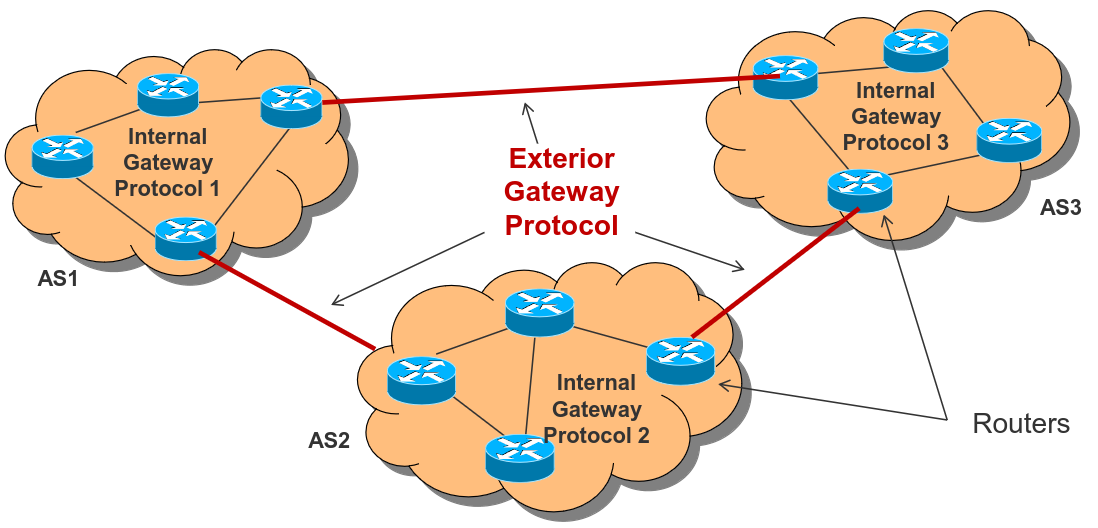
\includegraphics[scale=.3]{internet}
\end{center}

\paragraph{RIP} The \textbf{Routing Information Protocol} was the first IGP used. It's based on \textbf{distance vector} and it's \textbf{packet}, \textbf{flat} and \textbf{proactive}.\\
RIP messages are sent every $30$ seconds as UDP datagrams and they contain up to $25$ entries of the routing table. The metric used for evaluation is the \textbf{hop-number}, with a maximum of $15$ ($16 = \infty$).\\\\
\textbf{RIPv2} introduced the support for \textbf{subnets}, \textbf{CIDR}, \textbf{authentication}, \textbf{multicast} and more, but still limiting the max number of hops to $15$.\\\\
\textbf{RIPng} is an extension of RIPv2 to support IPv6.

\paragraph{OSPF} \textbf{Open Shortest Path First} is an IGP based on \textbf{link-state} and it's \textbf{hierarchical}, \textbf{packet} and \textbf{proactive}. It supports many different metrics, load balancing, hierarchical systems and security mechanisms to protect routers from wrong information.\\
It has modular support for three categories of link layers:
\begin{itemize}
	\item \textbf{Point-to-point} links between routers
	\item \textbf{Broadcast networks}, mostly LANs
	\item \textbf{Multi-access networks} without broadcasting, e.g. packet switching WANs
\end{itemize}
Since it's hierarchical, there are four types of routers:
\begin{itemize}
	\item \textbf{Internal}: belong only to one area
	\item \textbf{Area-border}: connect two or more areas, thus part of the backbone
	\item \textbf{Backbone}
	\item \textbf{AS border}: connect to other autonomous systems
\end{itemize}
\begin{center}
	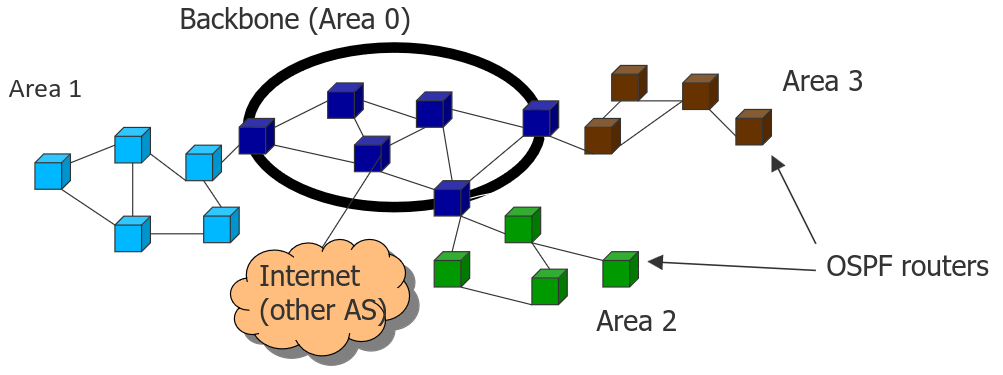
\includegraphics[scale=.3]{ospf}
\end{center}
Within an area every router has the same LSDB, while an \textit{area-border} one has LSDBs from each area it is connected to.

\paragraph{IS-IS} \textbf{Intermediate System to Intermediate System} it's a very similar IGP to OSPF, with the difference of being \textbf{neutral to layer 3 protocol} and thus getting faster support for IPv6. In this protocol, routers also build a \textbf{map of the network} to calculate the shortest path.\\
Has a lower overhead compared to OSPF and thus it's used in networks with a large number of routers.

\paragraph{BGP} In order to have an EGP, we need:
\begin{itemize}
	\item \textbf{Scalability}
	\item \textbf{Privacy}: networks want to hide their internal topologies
	\item \textbf{Policy enforcement}: networks need to control independently where to send and receive traffic
\end{itemize}
Thus, Distance Vector and Link State routing do not work, mainly because they agree on a common distance while Internet routing is much more diverse.\\\\
\textbf{Border Gateway Protocol} is a \textbf{path vector} protocol. BGP routers exchange \textbf{path vectors} with neighbors (\textbf{peers}), which then either accept or discard based on \textbf{policies}. Neighbors are typically connected directly or via switch but they can also be not topologically adjacent (\textbf{Multihop Peering}).

\begin{enumerate}
	\item BGP peers establish a TCP connection (\textbf{OPEN}, port 179) to exchange (\textbf{UPDATE}):
	\begin{itemize}
		\item \textbf{Network Layer Information}: prefixes
		\item \textbf{Paths}: list of AS numbers to reach a prefix
	\end{itemize}
	or to withdraw them. Two more messages exist: \textbf{KEEPALIVE} to check if adjacent peers are still available and \textbf{NOTIFICATION} to handle errors.
	\item BGP router collects all paths and stores them in the \textbf{Routing Information Base}
	\item Based on local policies and attributes a \textbf{preference} is assigned to all RIB entries
	\item For each IP prefix select one best route, choosing \textit{preference} over \textit{shortest path}
	\item Before announcing entries to the neighbors, filter based on \textbf{local policies}, which can be
	\begin{itemize}
		\item \textbf{Selection}: controls outbound traffic, specifying which path to use (e.g. customers over peers)
		\item \textbf{Export}: controls inbound traffic, specifying which path to advertise
	\end{itemize}
\end{enumerate}

\begin{note}
	Each AS appends itself when propagating announcement.
\end{note}

\begin{note}
	To debug BGP, \textbf{Looking Glasses} and \textbf{Routing Information Services} are used, giving you access to routing tables of BGP routers.
\end{note}

\begin{note}
	The duty of AS operators is to ensure \textbf{reachability} of their IP addresses or the IP addresses of their customers. There are two types of relations:
	\begin{itemize}
		\item \textbf{Customer-Provider}: the customer pays provider to get Internet connectivity. Usually records every 5 minutes the number of bytes sent and at the end of the month they bill in respect to the 95th percentile of the records
		\item \textbf{P2P Peering}: peers don't pay each other
	\end{itemize}
\end{note}

BGP has a lot of \textbf{problems}: \textbf{stability}, \textbf{routing table growth}, \textbf{load-balancing}, \textbf{hijacking}, but most of all \textbf{security}. While BGP peering sessions can be encrypted, they cannot be verified since the protocol is based on mutual trust.
\newpage
\subsection{Multicast}
\begin{wrapfigure}[12]{r}{3.5cm}
	\vspace{-1cm}
	\begin{center}
		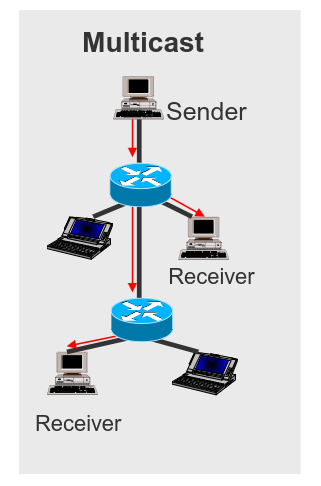
\includegraphics[width=3.5cm]{multicast2}
	\end{center}
\end{wrapfigure}
Group communication is used in multiple contexts, such as voice and video conferencing, content broadcasting (IPTV), games, etc..\\\\
Among the different types of communication, \textbf{multicast} is the most efficient to transmit to $n>1$ stations while sending the data only once. Multicast addresses a group of hosts based on a \textbf{single group address}, enabling the sender to deliver the data without knowing the receiving hosts.\\\\
The main idea is to use a \textbf{publish/surprise} paradigm, where the sender publishes independently of the receivers, which subscribes to the data independently of the first. The major protocols are \textbf{Internet Group Management Protocol} for IPv4 and \textbf{Multicast Listener Discovery} for IPv6.\\\\
There are two types of multicast:
\begin{itemize}
	\item \textbf{Any Source Multicast}: receive what anybody sends to the group without knowing the sources
	\item \textbf{Source Specific Multicast}: receive only what a specified source sends, explicitly selecting it and filtering
\end{itemize}

\subsubsection{Subscription}
We need a group subscription mechanism to reduce broadcasts, meaning that we want \textbf{switches} that know which ports belong to a certain group and \textbf{routers} that know about receivers to establish dynamic routing states.\\\\
MLD and IGMP messages are encapsulated into IP packets and are used between receivers and routers. When a receiver subscribes to a group, it informs the router about the interest. Then, periodically, the routers ask which groups are still present. If at all, they switch to only listen IGMP and MLD messages.

\subsubsection{IGMP}
IGMP is a protocol for delivery of multicast messages to all group members that are located in different physical networks. For this, routers need information about \textbf{group associations}.\\
If groups are only \textbf{temporary}, routers have to acquire information about associated hosts by themselves. With  IGMP messages, a multicast receiver subscribes to a group and thus informs routers about group interest, which periodically asks (\textbf{polling}), which groups of multicast are still present.\\
Routers exchange information to build \textbf{multicast routing trees} (routing protocol).\\\\
The creation of a \textbf{distribution tree} can be done in different ways:
\begin{itemize}
	\item \textbf{Flooding and Pruning} (Distance Vector Multicast Routing Protocol): it first floods multicast packets to all neighbors and the uses \textbf{Reverse Path Forwarding} to prevent loops
	\item \textbf{Protocol Independent Multicast}: it does not require a specific unicast protocol and can work in two modes
	\begin{itemize}
		\item \textbf{Dense}: like DVMRP
		\item \textbf{Sparse}: can support Internet-wide groups and explicitly constructs a tree using \textbf{rendezvous points}
	\end{itemize}
\end{itemize}

\newpage
\paragraph{PIM} Assuming that a low percentage of nodes will subscribe to a multicast group, we have:
\begin{itemize}
	\item \textbf{Receiver} will join a group through an IGMP Join in the local subnet and then PIM Join to a rendezvous point
	\item \textbf{Sender} does a PIM Join with the rendezvous point and sends them a register message. Then it distributes data along the multicast tree
\end{itemize}
\begin{center}
	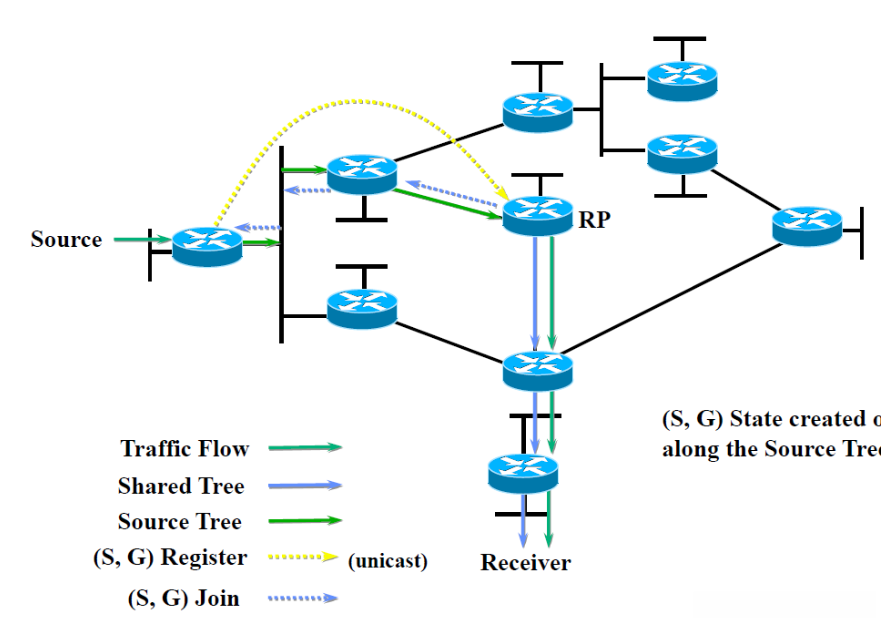
\includegraphics[scale=.4]{pimreg}
\end{center}

\subsubsection{API}
The multicast API uses Berkley sockets and has:
\begin{itemize}
	\item \textbf{IP\_ADD\_MEMBERSHIP} to join a group on a specific interface
	\item \textbf{IP\_DROP\_MEMBERSHIP} to leave a group (IGMPv2)
	\item \textbf{IP\_MULTICAST\_IF} to set or get default interfaces for use with multicast sends
	\item \textbf{IP\_MULTICAST\_LOOP} to disable loopback of outgoing multicast diagrams
	\item \textbf{IP\_MULTICAST\_TTL} to set the IP TTL of outgoing multicast datagrams
\end{itemize}

\subsubsection{Real applications}
Multicast is mainly used in \textbf{intra-domain} contexts (e.g. ISPs) due to IPTV, gaming, etc...\\
There is very limited development in the \textbf{inter-domain} context due to:
\begin{itemize}
	\item Difficult to achieve globally scalable routing
	\item No economic incentives for ISPs
\end{itemize}

\begin{note}
	In the \textbf{mobile} context, routing gets more complex due to the publish/subscribe approach of multicast.
\end{note}